\section{Banregler} \label{banregler}

Banan är uppmärkt med en tejp som är mellan 14-18mm tjock. Banan får korsa sin egen väg, med restriktionen att det skall ske rätvinkligt. Där banan korsar sin egen väg skall den vara rak i minst 30cm från korsningen. Avbrott i banan får förekomma, under förutsättning att det sker på en raksträcka och avbrottet inte är längre än 10 cm. Banans svängradie får ej understiga 25cm. \\
En station är markerad med en tejp vinkelrät mot banan åt det håll på vilket paket finns eller skall lämnas. Paketet ligger centrerat mot den vinkelräta tejpens ände. \\
En slutmarkering är inte nödvändig för banans giltighet. Finns det ett stopp markeras det av tre parallella tejpbitar på den sida på vilken robotens förvaringsutrymme finns. \\

\begin{figure}[h]
\center
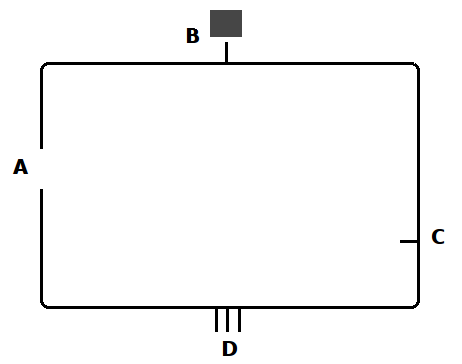
\includegraphics[scale=0.6]{grafik/kravspec-bana.png}
\endcenter
\caption{Exempelbana. Punkt A i figuren visar en upplockningsstation, B en station där ett paket finns, C en tom station och D ett stopp.}
\end{figure}
